
\documentclass[12pt]{article}
\usepackage[UTF8]{ctex}
\usepackage{geometry,booktabs,longtable,graphicx,amsmath}
\geometry{a4paper,margin=2.2cm}
\graphicspath{{../figures/}}
\title{A题：绿电直连型电氢氨园区优化运行}
\author{Codex 自动建模求解}
\date{2026年5月}
\begin{document}
\maketitle
\section*{摘要}
本文围绕绿电直连型电氢氨园区建立统一小时级功率平衡模型。所有问题严格使用题面给出的三项绿电直连指标：
\[
r_1=\frac{E_{use}-E_{sell}-E_{buy}}{E_{re}},\quad
r_2=\frac{E_{re}-E_{sell}}{E_{use}},\quad
r_3=\frac{E_{sell}}{E_{re}}.
\]
达标判定采用严格不等式：$r_1>60\%$、$r_2>30\%$、$r_3<20\%$。

\section{模型口径}
36 吨/日基础产能下，ALK、PEM 与合成氨装置额定功率分别为 10MW、10MW、0.75MW；扩容到 72 吨/日时三类设备同步线性放大，风电 40MW、光伏 64MW 和常规负荷不随产能放大。ALK、PEM 与合成氨装置按额定功率比例同步调节，避免模型偏向某一类电解槽。全年按 24 个场景各代表 15 天形成 360 天代表年。

\section{问题一结果}
典型日新能源发电量为 603.45 MWh，总用电量为 558.72 MWh，购电量为 172.04 MWh，上网电量为 216.77 MWh。三项指标分别为 0.282、0.692、0.359，达标分类为 partial。综合吨氨成本为 4368.63 元/吨。
\begin{figure}[htbp]\centering
\includegraphics[width=0.92\textwidth]{fig_problem1_power.png}\caption{问题一典型日功率曲线}\end{figure}

\section{问题二结果}
离散开停机模型中，开机小时按 72 吨/日产能满负荷运行，停机小时功率为 0。典型日最低综合吨氨成本对应日产量为 36 吨，成本为 3284.27 元/吨，达标分类为 partial。
\begin{figure}[htbp]\centering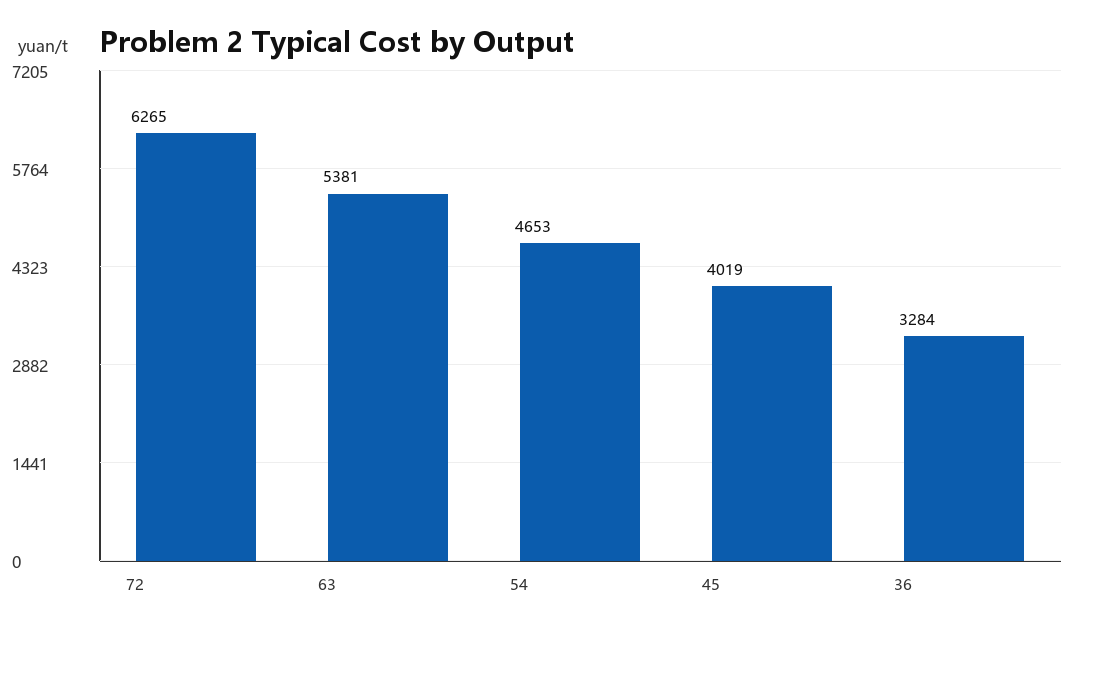
\includegraphics[width=0.9\textwidth]{fig_problem2_typical_cost.png}\caption{问题二典型日不同产量成本}\end{figure}

\section{问题三结果}
连续调节模型对每个给定日产量分别求解，日产氨量作为等式约束。24 场景代表年中，最低年平均综合吨氨成本对应日产量为 36 吨，年平均成本为 4304.55 元/吨。
\begin{figure}[htbp]\centering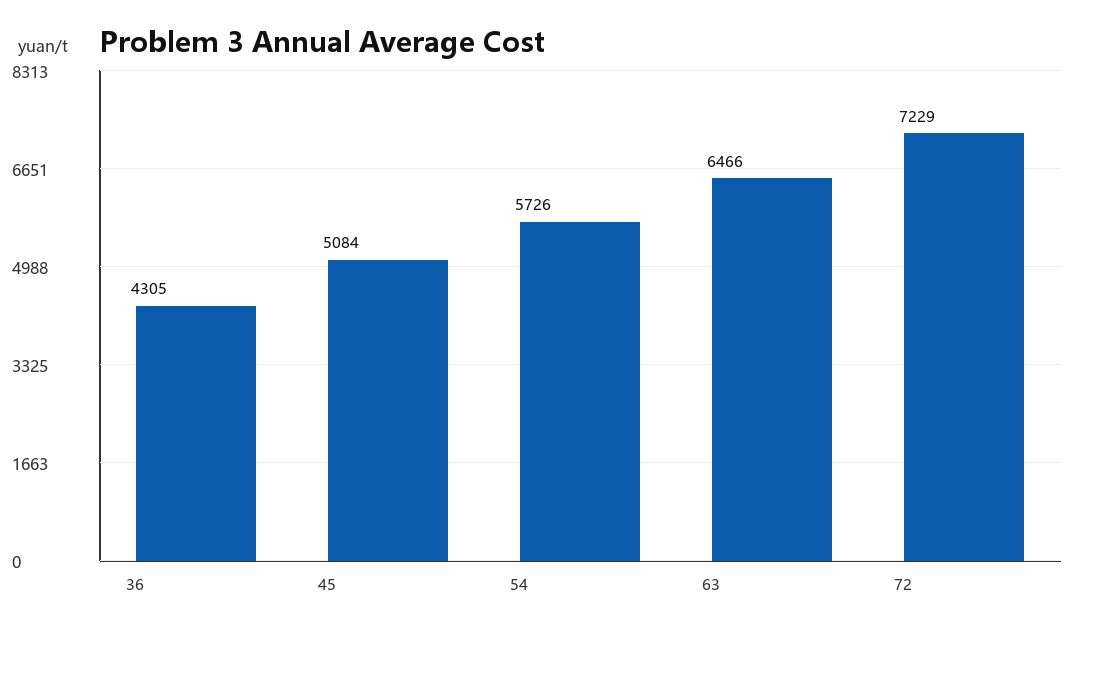
\includegraphics[width=0.9\textwidth]{fig_problem3_annual_cost.png}\caption{问题三不同产量代表年平均成本}\end{figure}

\section{问题四结果}
离网无储能阶段先最大化制氨量，再比较综合成本。最大弃电场景由无储能离网结果识别，为 风电场景4-光伏场景1。储能配置采用 $E_{bat}=20.0$ MWh、$P_{bat}=5.0$ MW，回放 24 场景后代表年产氨量为 10044.43 吨，年平均综合吨氨成本为 4246.01 元/吨。
\begin{figure}[htbp]\centering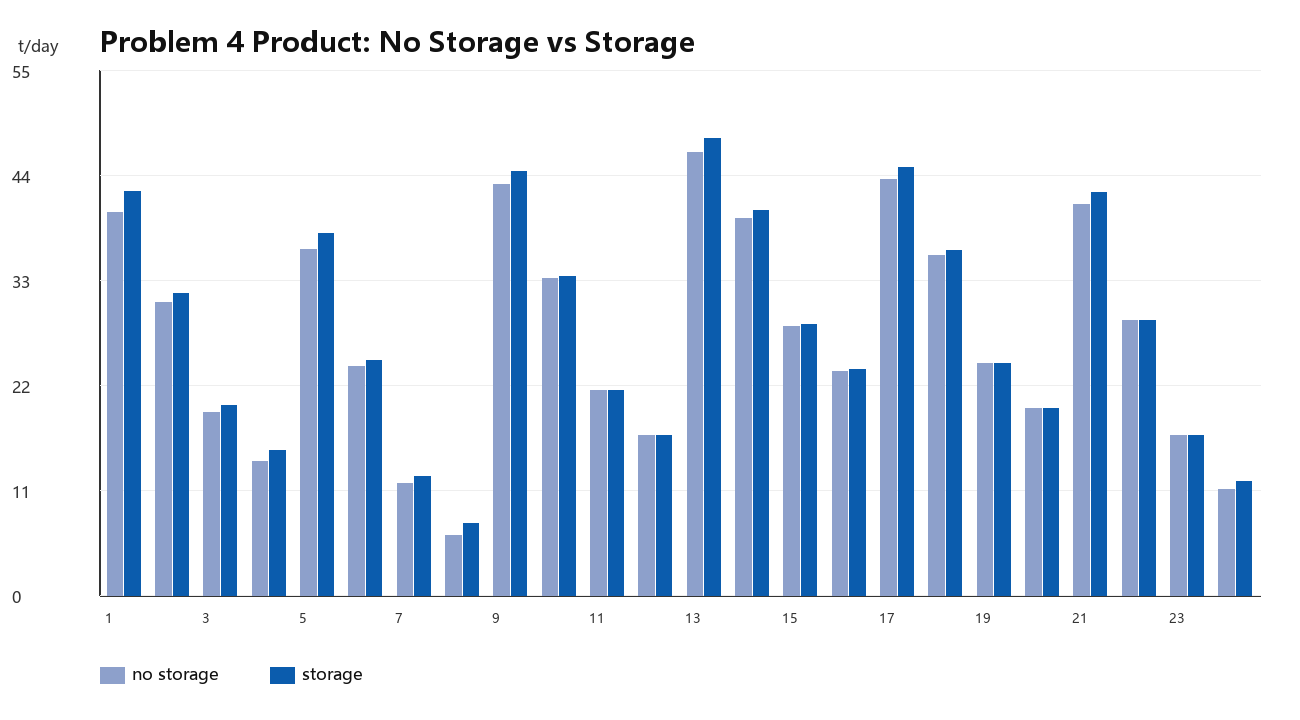
\includegraphics[width=0.9\textwidth]{fig_problem4_storage_compare.png}\caption{问题四储能前后产量对比}\end{figure}

\section{问题五政策分析}
绿电直连园区高渗透率提高后，一方面有利于新能源就近消纳、降低化工产品碳足迹、形成源荷储协同示范；另一方面也可能加剧局部电网潮流波动、调峰备用需求和结算边界复杂度。建议围绕以荷定源、储能与柔性负荷协同、多用户园区化交易、绿氨产品认证和辅助服务补偿机制完善政策体系。

\section{结论}
本求解采用统一数据、指标与成本函数，避免题面指标和政策指标混用。结果显示，离散和连续调节的核心差异来自生产小时可选性和功率柔性，储能在离网模式下主要通过吸收弃电提升产量，但其经济性依赖容量成本与目标产量约束。
\end{document}
